% !TEX TS-program = XeLaTeX
% use the following command:
% all document files must be coded in UTF-8
\documentclass[portuguese]{textolivre}
% build HTML with: make4ht -e build.lua -c textolivre.cfg -x -u article "fn-in,svg,pic-align"

\journalname{Texto Livre}
\thevolume{19}
%\thenumber{1} % old template
\theyear{2026}
\receiveddate{\DTMdisplaydate{2025}{7}{6}{-1}} % YYYY MM DD
\accepteddate{\DTMdisplaydate{2025}{10}{3}{-1}}
\publisheddate{\DTMdisplaydate{2025}{12}{2}{-1}}
\corrauthor{Ana Emília Klein}
\articledoi{10.1590/1983-3652.2026.60146}
%\articleid{NNNN} % if the article ID is not the last 5 numbers of its DOI, provide it using \articleid{} commmand 
% list of available sesscions in the journal: articles, dossier, reports, essays, reviews, interviews, editorial
\articlesessionname{articles}
\runningauthor{Faleiro e Klein} 
%\editorname{Leonardo Araújo} % old template
\sectioneditorname{Daniervelin Pereira~\orcid{0000-0003-1861-3609}}
\layouteditorname{Leonardo Araújo~\orcid{0000-0003-3884-2177}}

\title{A estilística genérica em produções de texto acadêmicas assistidas por Inteligência Artificial Generativa}
\othertitle{Generic stylistics in academic text production assisted by Generative Artificial Intelligence}
% if there is a third language title, add here:
%\othertitle{Artikelvorlage zur Einreichung beim Texto Livre Journal}

\author[1]{Róger Sullivan Faleiro~\orcid{0000-0003-4136-839X }\thanks{Email: \href{mailto:rfaleiro@mx2.unisc.br}{rfaleiro@mx2.unisc.br}}}
\author[2]{Ana Emília Klein~\orcid{0009-0005-8833-4877}\thanks{Email: \href{mailto:aeklein@univates.br}{aeklein@univates.br}}}
\affil[1]{Universidade de Santa Cruz do Sul, Santa Cruz do Sul, RS, Brasil.}
\affil[2]{Universidade do Vale do Taquari, Curso de Letras, Lajeado, RS, Brasil.}

\addbibresource{article.bib}
% use biber instead of bibtex
% $ biber article

% used to create dummy text for the template file
\definecolor{dark-gray}{gray}{0.35} % color used to display dummy texts
\usepackage{lipsum}
\SetLipsumParListSurrounders{\colorlet{oldcolor}{.}\color{dark-gray}}{\color{oldcolor}}

% used here only to provide the XeLaTeX and BibTeX logos
\usepackage{hologo}

% if you use multirows in a table, include the multirow package
\usepackage{multirow}

% provides sidewaysfigure environment
\usepackage{rotating}

% CUSTOM EPIGRAPH - BEGIN 
%%% https://tex.stackexchange.com/questions/193178/specific-epigraph-style
\usepackage{epigraph}
\renewcommand\textflush{flushright}
\makeatletter
\newlength\epitextskip
\pretocmd{\@epitext}{\em}{}{}
\apptocmd{\@epitext}{\em}{}{}
\patchcmd{\epigraph}{\@epitext{#1}\\}{\@epitext{#1}\\[\epitextskip]}{}{}
\makeatother
\setlength\epigraphrule{0pt}
\setlength\epitextskip{0.5ex}
\setlength\epigraphwidth{.7\textwidth}
% CUSTOM EPIGRAPH - END

% to use IPA symbols in unicode add
%\usepackage{fontspec}
%\newfontfamily\ipafont{CMU Serif}
%\newcommand{\ipa}[1]{{\ipafont #1}}
% and in the text you may use the \ipa{...} command passing the symbols in unicode

% LANGUAGE - BEGIN
% ARABIC
% for languages that use special fonts, you must provide the typeface that will be used
% \setotherlanguage{arabic}
% \newfontfamily\arabicfont[Script=Arabic]{Amiri}
% \newfontfamily\arabicfontsf[Script=Arabic]{Amiri}
% \newfontfamily\arabicfonttt[Script=Arabic]{Amiri}
%
% in the article, to add arabic text use: \textlang{arabic}{ ... }
%
% RUSSIAN
% for russian text we also need to define fonts with support for Cyrillic script
% \usepackage{fontspec}
% \setotherlanguage{russian}
% \newfontfamily\cyrillicfont{Times New Roman}
% \newfontfamily\cyrillicfontsf{Times New Roman}[Script=Cyrillic]
% \newfontfamily\cyrillicfonttt{Times New Roman}[Script=Cyrillic]
%
% in the text use \begin{russian} ... \end{russian}
% LANGUAGE - END

% EMOJIS - BEGIN
% to use emoticons in your manuscript
% https://stackoverflow.com/questions/190145/how-to-insert-emoticons-in-latex/57076064
% using font Symbola, which has full support
% the font may be downloaded at:
% https://dn-works.com/ufas/
% add to preamble:
% \newfontfamily\Symbola{Symbola}
% in the text use:
% {\Symbola }
% EMOJIS - END

% LABEL REFERENCE TO DESCRIPTIVE LIST - BEGIN
% reference itens in a descriptive list using their labels instead of numbers
% insert the code below in the preambule:
%\makeatletter
%\let\orgdescriptionlabel\descriptionlabel
%\renewcommand*{\descriptionlabel}[1]{%
%  \let\orglabel\label
%  \let\label\@gobble
%  \phantomsection
%  \edef\@currentlabel{#1\unskip}%
%  \let\label\orglabel
%  \orgdescriptionlabel{#1}%
%}
%\makeatother
%
% in your document, use as illustraded here:
%\begin{description}
%  \item[first\label{itm1}] this is only an example;
%  % ...  add more items
%\end{description}
% LABEL REFERENCE TO DESCRIPTIVE LIST - END


% add line numbers for submission
%\usepackage{lineno}
%\linenumbers

\begin{document}
\maketitle

\begin{polyabstract}
\begin{abstract}
Este artigo investiga o uso da Inteligência Artificial Generativa na produção de textos por estudantes do ensino superior, com foco no contexto do ensino a distância, dado que esse cenário tem se constituído como um desafio para a manutenção da qualidade da aprendizagem. Para isso, realizou-se uma análise, a partir da Teoria da Linguística Textual, de resenhas acadêmicas produzidas em um componente curricular ofertado na modalidade EAD. Como resultado, observaram-se similaridades entre os textos, as quais foram classificadas em duas categorias: “repetição de palavras” e “encadeamento sintático e combinações fixas”, que podem servir de base para a identificação de textos assistidos por IAG. Conclui-se que, embora sem uma análise detalhada possam ser considerados inéditos, textos gerados nessas condições apresentam estruturas recorrentes que frequentemente funcionam como fórmulas esvaziadas de sentido, configurando, assim, produções distantes dos objetivos formativos relacionados ao desenvolvimento da autoria e da reflexão crítica em estudantes universitários.

\keywords{Linguística \sep Linguagem acadêmica \sep Processos de escrita \sep Inteligência Artificial \sep Educação a distância}
\end{abstract}

\begin{english}
\begin{abstract}
This paper investigates the use of General Artificial Intelligence in text production by university students, with a focus on the context of distance education, since this scenario has been a challenge for maintaining the quality of learning. To this end, an analysis was carried out, based on Theory of Text Linguistics, of academic reviews written in a distance learning curricular course. The results showed similarities among the texts, which were classified into two categories: “repetition of words” and “syntactic linking and fixed combinations”, useful for identifying texts assisted by IAG. The conclusion is that although without a detailed analysis they could be considered unpublished, texts generated under these conditions have recurring structures that often function as formulas emptied of meaning, thus constituting productions that are far removed from the formative objectives related to the development of authorship and critical reflection in university students.

\keywords{Linguistics \sep Academic language \sep Writing processes \sep Artificial Intelligence \sep Distance education}
\end{abstract}
\end{english}
% if there is another abstract, insert it here using the same scheme
\end{polyabstract}

\section{Introdução}\label{sec-intro}
Em um contexto de precarização das relações de trabalho e de redução do poder aquisitivo das classes trabalhadoras, o ensino superior a distância (EAD) emerge como uma alternativa viável para muitos brasileiros. Inicialmente voltada para atender necessidades específicas de qualificação profissional, a educação a distância expandiu-se significativamente entre 2010 e 2020, período em que houve um aumento de 474\% no número de ingressantes em cursos superiores nessa modalidade, enquanto o ingresso em graduações presenciais diminuiu 16,5\% entre 2020 e 2021 \cite{INEP2025}. Esse cenário levou universidades, especialmente as privadas e as comunitárias, a se adaptar a essa modalidade investindo em cursos EAD para manter sua sustentabilidade diante da significativa evasão de estudantes dos cursos presenciais. Se alguns sistemas de ensino priorizam a eficiência operacional (para não dizer os lucros), essas questões não ficam restritas a eles: mesmo as universidades mais tradicionais do país, ou aquelas que prezam pela educação de qualidade, são obrigadas a se submeter a essa nova forma de ensino devido às consequências da aceleração do capital para cima das universidades que, se ainda não foram destruídas, têm em seus \textit{campi} a diminuição no número de estudantes.

Decorre disso a precarização do trabalho do professor/tutor, que, dentro dessa realidade, passa a atender turmas cada vez maiores, já que as salas de aula virtuais e o material didático (como textos interativos, vídeos e objetos digitais de aprendizagem) podem ser acessados por muitos estudantes ao mesmo tempo. A massificação da modalidade, embora possa ser um alívio financeiro para algumas universidades em termo de contas, desafia o professor/tutor no acompanhamento\footnote{Expressão característica da EAD que substitui o processo pedagógico construído de forma dialógica no presencial, com a interação entre professor e estudante. Na EAD, a experiência, muito menos colaborativa e muito mais solitária, exige um monitoramento constante da entrega das atividades e notas obtidas pelos estudantes.} do estudante, pois os encontros síncronos costumam ser reduzidos e parte-se do pressuposto de que o estudante deve administrar seu aprendizado, interagindo com os conteúdos de forma adequada e satisfatória; isto é, o desenvolvimento do aluno depende do seu próprio esforço.

Soma-se a isso o impacto da tecnologia, que é essencial para que o modelo EAD aconteça e, por isso, também transforma as dinâmicas de ensino e aprendizagem, tanto no sentido de possibilitá-las quanto de limitá-las. Mais recentemente, a emergência de aplicações de inteligência artificial generativa (IAG), como o ChatGPT, tem impactado a educação e sido tema de debate. A ferramenta é festejada como promessa de produtividade, algo desejado na cultura de aceleração e competição presente na educação – não apenas no que diz respeito a educadores sobrecarregados de trabalho, mas também entre os alunos. Por um lado, o ChatGPT pode ser uma ferramenta para a criação e a lapidação de ideias, auxiliando os estudantes na organização de pensamentos, estruturação inicial de textos acadêmicos ou, ainda, na revisão final; por outro, o uso indiscriminado desse recurso pode distanciar ainda mais o aluno de um aprendizado mais ativo, uma vez que essa tecnologia permite acessar respostas rápidas, produzir textos e até realizar tarefas inteiras com facilidade, sem olhar crítico frente às atividades propostas ao longo do curso.

Nesse sentido, este artigo busca analisar o uso da IA generativa pelos estudantes da modalidade EAD de uma universidade comunitária, especificamente em tarefas de produção textual escrita no componente curricular \textit{Leitura e Escrita de Textos Acadêmicos: Produção Reflexiva, Crítica e Criativa}. Partimos do questionamento sobre as práticas avaliativas tradicionais, que, em muitos casos, se mostram vulneráveis às tecnologias que substituem a participação ativa dos estudantes no processo de aprendizado, especialmente em componentes curriculares que envolvem leitura e produção de textos acadêmicos, em que a utilização indiscriminada da IAG ameaça ainda mais o propósito formativo. À luz da Linguística Textual, o estudo investiga as características e as similaridades estruturais que podem indicar o uso de inteligência artificial na produção de textos submetidos à avaliação pelos estudantes do ensino superior. Com isso, pretendemos discutir o impacto do uso de IAG no propósito formativo do componente curricular e as tentativas já realizadas pelos autores de mitigar o uso desse recurso, a fim de promover maior qualidade de ensino e desenvolvimento cognitivo do estudante.

\section{Por que e como escrevemos textos acadêmicos?}\label{sec-normas}
\subsection{O ato de escrever textos autênticos}
A habilidade de escrever não é inata ao ser humano. Diante disso, há a necessidade de aprendê-la a partir de uma sequência de estratégias que perpassam a identificação de códigos em sons e atribuir, através das suas respectivas combinações, significados. A habilidade de escrever, assim como de ler e compreender um texto, possui diferentes níveis que se embasam na capacidade de o sujeito utilizar seu léxico para construir orações e conectar suas ideias de forma coesa e coerente, a fim de comunicar sua mensagem de forma clara para que o leitor a compreenda. Logo, escrever é uma competência que se desenvolve através de diversos processos que requerem domínio da língua, atenção e prática. O processo de aprender a escrever, nesse sentido, inicia-se nos primeiros anos da vida escolar do sujeito, a partir do processo de alfabetização e se prolonga até o ensino médio, quando o estudante deve apresentar a capacidade de ler de forma crítica \cite{Morais2013}, entender o funcionamento da língua portuguesa e, logo, produzir textos com autonomia.

De acordo com a perspectiva adotada neste artigo, entendemos que um texto não é uma mera extensão da frase ou um conjunto de frases, mas constitui uma unidade de sentido, como um “tecido estruturado, uma entidade significativa, uma entidade de comunicação e um artefato histórico. De certo modo, pode-se afirmar que o texto é uma (re)construção do mundo [do enunciador]” \cite[p. 72]{Marcuschi2008}. Portanto, o processo de escrita de textos se fundamenta na capacidade de o sujeito encadear suas ideias, de modo que estrutura não pode ser considerada simplesmente uma combinação aleatória de frases, e sim uma sequência de decisões que buscam alcançar um objetivo comunicativo. \textcite[p. 22]{Koch1995} corrobora essa concepção afirmando que o texto é um ato consciente e se constitui como uma tarefa “criativa, que compreende o desenvolvimento de estratégias concretas de ação e de escolha por meios adequados à realização dos objetivos” que orbitam na intencionalidade daquele que o produz e na compreensão daquele que o recebe.

Diante disso, com base no processo que é orquestrado para o ensino da escrita como um ato enunciativo que envolve habilidades sofisticadas, espera-se que o estudante de nível superior já possua essa bagagem consolidada e esteja apto a ler, compreender e produzir diferentes tipos de textos, assim como desenvolver a capacidade de interagir com e produzir textos nos gêneros propriamente acadêmicos. Nesse sentido, no início dessa etapa, procura-se ofertar componentes curriculares que revisitam alguns conceitos conhecidos no ensino médio para, em seguida, adentrar em conteúdos específicos da academia, como a elaboração de resenhas críticas – que são as produções discentes analisadas neste artigo.

Esse gênero textual, como qualquer outro, apresenta uma estrutura que pode, de certa forma, ser engessada, mas é também ela que permite seu próprio reconhecimento enquanto gênero. Assim, embora possua elementos comuns, como a apresentação do texto resenhado, sua análise e sua crítica, cada autor é livre para adotar diferentes abordagens com base na sua perspectiva como sujeito/resenhista. Logo, ainda que os gêneros textuais apresentem uma forma característica, a resenha crítica pode (e, inevitavelmente, deve) apresentar variações – de organização, criticidade, estilística, entre outras – que estão à mercê da criatividade e da bagagem linguística do autor, no caso, do estudante, aspectos esses que refletem e impactam na criação de um texto propriamente autêntico.

Ainda no que concerne à produção de textos acadêmicos, vale um destaque: o respeito à propriedade intelectual das fontes utilizadas e à originalidade das ideias é esperado nesse contexto. É por isso que componentes curriculares que envolvem leitura e produção de textos são enfáticos sobre a importância de estudantes citarem corretamente os autores consultados, além de elaborarem paráfrases que não distorçam as ideias referenciadas. Sendo o plágio uma violação grave da ética acadêmica, especialmente quando envolve a apropriação de ideias sem autorização e sem a devida atribuição por meio da cópia direta ou não dos discursos, a questão da definição clara da autoria de um texto é um assunto relevante no meio universitário e deve ser considerada quando se propõem práticas de escrita desse gênero.

\subsection{O que significa escrever: a recursividade humana e a probabilidade da IAG}\label{sec-conduta}
A recursividade é uma propriedade fundamental da linguagem humana \cite{Battisti2021}. No caso do português brasileiro, cuja gramática e vocabulário – vasto, ainda que finito – são compartilhados entre os falantes da língua, é possível criar tantas sentenças distintas que acreditamos na infinitude de produção de textos. Essa característica também permite uma pluralidade de estilos de escrita, que podem ser adotados conforme a intenção e a situação comunicativa, de modo que alguns são, inclusive, reconhecidos: estilo kafkiano, machadiano, roseano. A recursividade também possibilita ineditismo, talvez ninguém tenha dito/escrito até hoje a frase “um canguru pulou no meu artigo”, por exemplo, e se o fez, não foi uma cópia o que escrevemos aqui, mas uma casualidade. O fato é que uma criança, ao aprender a língua materna, não o faz simplesmente reproduzindo palavras e frases que ouve; ela pode, a partir da gramática internalizada, criar frases inéditas no seu contexto.

Entretanto, quando se trata de produção textual assistida por inteligência artificial generativa (IAG) – uma tecnologia que pretende simular a inteligência humana na geração de conteúdo de texto, imagem, áudio etc. – o processo não se dá por meio da recursividade, mas opera com base em probabilidade. Conforme explica \textcite{Santaella2023}, o ChatGPT\footnote{Neste estudo, concentramo-nos especificamente no ChatGPT por ser a ferramenta de IAG mais conhecida e usada entre os estudantes universitários para a produção de textos acadêmicos.} gera conteúdos a partir de uma base de textos de bilhões de páginas da web, não a partir da totalidade de textos existentes, mas de uma lista de termos que provavelmente apareceriam na sequência um do outro. O chatbot emprega a palavra mais frequente, entendendo que ela será mais acessível ao leitor comum, o que lhe permite a criação de textos aparentemente originais, com elementos em uma disposição sempre nova. Esse funcionamento, contudo, levanta questionamentos sobre a natureza da “criatividade” da IAG e suas limitações em relação à produção textual humana, uma vez que esse mesmo cálculo poderia limitar a produção de textos verdadeiramente autênticos.

A “democratização do acesso a esses produtos tecnológicos – e a consequente possibilidade de utilizá-los para a obtenção de informações [e, acrescentamos, realização de tarefas] – é um grande desafio para a sociedade atual e demanda esforços e mudanças nas esferas econômicas e educacionais” \cite[p. 22]{Kenski2013}. No contexto da educação, alguns defendem a inevitabilidade da IAG sugerindo que a mudança precisa ocorrer nas atividades propostas\footnote{Esta visão é comumente compartilhada nos corredores universitários entre os docentes como uma forma de “contornar” o uso do ChatGPT por parte dos estudantes.}: é preciso formular tarefas que dificultem o uso da tecnologia, de maneira que o estudante não consiga obter respostas prontas ao recorrer ao ChatGPT. À primeira vista, podemos concordar com essa afirmativa, pois isso poderia encaminhar para atividades mais aproximadas da realidade do estudante, por exemplo. Todavia, pensemos em um componente curricular que, sob diferentes nomes, costuma figurar na grade curricular dos cursos de graduação e tem como objetivo introduzir os estudantes na leitura e escrita de textos acadêmicos. Será que, nesse caso, faz sentido que o problema esteja na formulação da atividade? Uma resposta afirmativa apenas pode ser dada se assumirmos que habilidades cognitivas, como ler e escrever, deixarão de ser necessárias – assim como a força humana que vem sendo historicamente substituída por máquinas – uma vez que os \textit{chatbots} podem desempenhá-las com “eficácia”. Tal estágio, ao que parece, ainda não foi alcançado.

Este artigo não pretende apresentar o uso da IAG de uma perspectiva dicotômica, pesando seus benefícios e prejuízos, mas problematizar o uso desse recurso pelos estudantes que simplificam ao máximo as atividades acadêmicas, negligenciando sua responsabilidade no processo de ensino-aprendizagem. \textcite[p. 26]{Kenski2013} observa que a “tecnologia moderna reestrutura ainda mais profundamente a consciência e a memória, impondo uma nova ordem nos nossos modos de compreender e de agir sobre o mundo”. A partir disso, podemos nos perguntar: será que a tecnologia realmente direciona o ser humano para a sua melhor performance? Estamos nós, enquanto sociedade, ainda buscando cultivar competências que promovam a autonomia intelectual e crítica em um contexto em que as máquinas desempenham papéis complementares e não substitutivos? Se a resposta a essa última questão for um “sim”, não seria o caso de, em vez de simplesmente nos adaptarmos às tecnologias, repensar os processos educacionais frente à realidade vivenciada e procurar formas de estimular a aprendizagem ainda que isso signifique recorrer a práticas pedagógicas mais “analógicas”?


\section{Metodologia}\label{sec-fmt-manuscrito}
Esta pesquisa é caracterizada como quanti-qualitativa \cite{Gil2002} e tem como objetivo investigar o uso de Inteligência Artificial em atividades de produção textual de estudantes de graduação na EAD. Para isso, foi selecionada uma das principais atividades avaliativas de escrita do componente curricular \textit{Leitura e Escrita de Textos Acadêmicos: Produção Reflexiva, Crítica e Criativa}, que se caracteriza por abranger os estudantes universitários de todos os cursos de graduação (bacharelado e licenciatura) e tecnólogos oferecidos pela instituição pesquisada. Trata-se de uma disciplina obrigatória que costuma estar, se não no primeiro semestre, no primeiro ano dos cursos da instituição, uma vez que visa desenvolver habilidades relacionadas tanto à oralidade, quanto à leitura e à escrita de textos acadêmicos, com enfoque em gêneros textuais comuns nesse meio, como resumo, resumo de artigo científico, e-mail e resenha crítica.

A atividade relacionada à produção de uma resenha crítica foi escolhida para esta análise por ser uma das mais significativas do componente curricular, já que esse gênero textual pressupõe leitura e compreensão das ideias originais do(s) autor(es), capacidade de síntese e posicionamento crítico em relação ao conteúdo e à estrutura do texto resenhado. No caso pesquisado, a atividade ocorreu durante o mês de maio de 2024, em uma turma composta por 184 estudantes, sendo que 149 realizaram a entrega da resenha crítica solicitada, compondo o corpus deste estudo.

Após três semanas de estudo do gênero resenha crítica, os estudantes foram convidados a escreverem uma resenha autoral. Antes de iniciar a atividade, eles deveriam ler três textos, sendo eles: “Nada é possível; tudo é possível”, de Mário Sérgio Cortella e Leandro Karnal; “Para que estudar gramática?”, de Mário Perini; e “Vida Socializada”, de Clóvis de Barros Filho e Arthur Meucci – em seguida, deveriam selecionar o texto que considerassem mais interessante para a produção da resenha.

Ainda com o intuito de auxiliar os estudantes na organização do texto, foram explicitadas, no enunciado da atividade, quatro ações que deveriam constar na resenha: apresentar o capítulo; descrever; avaliar e recomendar a obra. No roteiro, também constava um aviso sobre plágio: “atenção: se houver, em seu texto, trechos copiados de outros textos sem que seja feita a citação adequada, isso será considerado plágio, e o trabalho será anulado. Assim, seu texto não receberá nota e não haverá possibilidade de reescrita”, acompanhado de uma cartilha sobre o assunto, elaborada pela \textcite{UFF2010}.

Durante a avaliação das resenhas, foram identificadas similaridades entre elas, o que culminou na investigação e identificação do uso de Inteligência Artificial na produção dos textos. Assim, a fim de dar conta do objetivo proposto neste artigo, os textos dos estudantes foram analisados à luz da Linguística Textual \cite{Marcuschi2008} com o intuito de identificar aspectos que pudessem apontar o uso de Inteligência Artificial. Para a análise dos dados, buscou-se verificar tais ocorrências especificamente nos parágrafos que pretendem avaliar e recomendar a obra. Com o intuito de organizar os achados, foram criadas duas categorias: “repetição de palavras” e “encadeamento sintático e combinações fixas”, apresentadas na sequência.


\section{Traços de IAG na escrita acadêmica}\label{sec-formato}
Antes de iniciarmos a análise, vale ressaltar que a universidade em questão conta com o Turnitin, uma ferramenta que identifica as similaridades entre o texto submetido e uma extensa base de dados que inclui publicações acadêmicas e outros conteúdos disponíveis on-line, além de um banco interno, composto por trabalhos de estudantes indexados na plataforma Moodle da instituição desde o ano 2022. Para cada texto analisado, a ferramenta gera um relatório que apresenta o percentual de similaridade com a base de dados e identifica as repetições de orações completas e a combinação de palavras em uma determinada sequência, vinculando-as à possível fonte. Desse modo, o avaliador pode analisar os dados a fim de descartar (ou não) a ocorrência de plágio. No corpus investigado, a aplicação indicou percentuais de similaridade que chegaram a 47\% entre as resenhas consideradas neste estudo.


\subsection{A gramática da IAG}\label{sec-modelo}
Como dito anteriormente, para esta análise, o estudo se deteve na identificação de similaridades nos parágrafos que objetivavam analisar e recomendar a obra. Os textos apresentados pelos estudantes revelaram uma série de padrões recorrentes de uso da língua, o que levantou a suspeita do uso de IA na produção das resenhas. Nesta subseção, apresentaremos os principais padrões identificados e os exemplos que corroboram os achados extraídos dos textos dos estudantes e destacados com recuo específico e em itálico. Para indicar aspectos diretamente no texto original, utilizamos o grifo com sublinhado, de forma a facilitar a visualização dos elementos analisados.

\subsubsection{Repetição de palavras}\label{sec-organizacao}
A primeira característica que chama a atenção de professores de língua portuguesa é a repetição de termos ou expressões que raramente aparecem em produções de estudantes. Essa percepção por parte dos professores de língua portuguesa, que também é o nosso caso, desenvolve-se ao longo da experiência docente e permite prever, em certa medida, a consciência linguística dos estudantes em diferentes momentos da vida.

A \Cref{tbl1} mostra a relação de palavras ou expressões que apareceram com frequência significativa nas resenhas analisadas e que, em virtude da posição que ocupam dentro das frases, estão entre as que mais despertaram interesse para esta pesquisa.


\begin{table}[h!]
\centering
\begin{threeparttable}
\caption{Padrões lexicais encontrados nas resenhas críticas}
\label{tbl1}
\begin{tabular}{ccc}
\toprule
\textbf{Termo/expressão} & \textbf{Resenhas} & \textbf{Ocorrências} \\
\midrule
acessível(is) & 41 & 56 \\
enriquece; enriquecedor/a & 36 & 56 \\
envolvente & 23 & 32 \\
insight(s) & 27 & 33 \\
insights valiosos & 15 & 15 \\
inspirador(a) & 23 & 33 \\
mas também & 33 & 38 \\
não apenas & 21 & 27 \\
não só & 18 & 21 \\
oferece/r & 56 & 85 \\
mergulhar & 8 & 8 \\
perspicaz & 14 & 18 \\
-profund- & 76 & 176 \\
profundas & 15 & 17 \\
provocativa & 12 & 15 \\
valioso(s)/a(s) & 28 & 36 \\
\bottomrule
\end{tabular}
\source{Dos autores (2025).}
\end{threeparttable}
\end{table}

Desde escolhas mais usuais como “profunda(s)”, contabilizando 86 ocorrências, até termos menos comuns, como “insight(s)”, com 33 ocorrências, e “valioso/a(s)”, com 36 ocorrências, ou ainda mais raros, como “insights valiosos”, com 15 ocorrências, essas expressões isoladas ou em combinações, como veremos mais adiante, destacam-se pela frequência com que são usadas nos textos analisados.

Para fins de comparação, termos esperados em grande número em uma resenha como “autor/a(es)” foram encontrados 480 vezes em 130 resenhas; enquanto um total de 41 estudantes classificaram o texto resenhado como “acessível” e 36 como “enriquecedor”. Além disso, vale observar o contraste entre verbos como “afirmar” (52 ocorrências) e “oferecer” (85 ocorrências). O primeiro é muito usado em textos acadêmicos, com o objetivo de introduzir argumentos ou ideias de outro autor, o que é esperado em resenhas acadêmicas. Já o verbo “oferecer” é uma escolha menos usual nesse gênero de texto, mas aparece de forma significativa no conjunto de resenhas, essa frequência elevada sugere um padrão discursivo específico, possivelmente influenciado por modelos textuais.

\subsubsection{Encadeamento sintático e combinações fixas}\label{sec-organizacao-latex}
Outro aspecto que chamou atenção nas resenhas foi a recorrência de determinadas construções sintáticas a partir de combinações fixas de palavras. Dentre essas, podemos destacar a estrutura “[substantivo] + ABORDAR + de forma abrangente”, frequentemente seguida pela expressão “papel crucial” na mesma oração, como podemos ver nos exemplos abaixo:

\begin{quote}
\itshape
Este capítulo \underline{da obra aborda de forma abrangente o papel crucial} desempenhado pela ciência e pela tecnologia [...]

\underline{O capítulo aborda o papel crucial da ciência e da tecnologia} na sociedade contemporânea [...]

\underline{Abordando de forma abrangente o papel crucial} da ciência, tecnologia e educação na sociedade contemporânea [...]
\end{quote}

Além do adjetivo “crucial”, observamos o uso de “profunda” para qualificar “reflexão” ou termos equivalentes. De maneira semelhante, o adjetivo “enriquecer” é frequentemente empregado para descrever a leitura. Exemplos disso podem ser observados a seguir:

\begin{quote}
\itshape
A riqueza dos argumentos apresentados e a \underline{profundidade das reflexões} oferecem uma visão panorâmica sobre a natureza humana e a dinâmica social.

O diálogo entre Cortella e Karnal proporciona uma experiência de aprendizado e introspecção única, capaz de inspirar uma \underline{profunda reflexão} sobre o sentido da existência e o papel da virtude e da vaidade em nossas vidas.

Com \underline{percepções profundas} e provocativas, este capítulo é uma fonte valiosa de reflexão e inspiração para qualquer um que busque uma jornada intelectual envolvente e enriquecedora [...]

Recomendar este livro é sugerir \underline{uma leitura que não só enriquece} intelectualmente, mas que também pode ter um impacto profundo na forma como o leitor vive e percebe sua própria existência.

A compreensão oferecida pelos autores são pertinentes e \underline{enriquecedoras} [...]

Compensa salientar, que é \underline{uma leitura que enriquece} nossa compreensão e instiga nossa moralidade, desenvolvendo nosso caráter, tornando-nos seres mais conscientes e virtuosos [...]
\end{quote}

Também identificamos uso expressivo de adjetivos e ocorrências de dupla adjetivação, em que os modificadores dos núcleos nominais aparecem coordenados por “e”. Esses pares de adjetivos geralmente assumem funções de núcleo do predicativo ou do adjunto adnominal e variam entre si, porém, ainda assim, é possível encontrar recorrências entre eles:

\begin{quote}
\itshape
Com percepções \underline{profundas e provocativas} [...]

O capítulo apresenta uma análise \underline{profunda e provocativa} [...]

[...] Os autores fornecem uma análise \underline{perspicaz e provocativa} [...]

A abordagem \underline{clara e provocativa} dos autores [...]

[...] os autores oferecem uma análise \underline{perspicaz e inspiradora} [...]

A obra oferece insights \underline{valiosos e inspiradores} [...]

A abordagem do autor neste capítulo é \underline{filosófica e prática}, tornando-o uma leitura \underline{envolvente} \underline{e aplicável} à vida cotidiana. Um de seus pontos fortes é o sucesso de Clóvis de Barros Filho e Arthur Meucci em traduzir conceitos filosóficos complexos em exemplos \underline{concretos e acessíveis}. Isso facilita a compreensão e a aplicação das ideias apresentadas.

A linguagem é \underline{acessível e envolvente}, tornando a filosofia uma ferramenta prática e útil na vida cotidiana.

[...] torna a leitura \underline{envolvente e acessível}.
\end{quote}

Outro aspecto diz respeito ao uso frequente do termo inglês “insight”, já mencionado na subseção 4.1.1., especialmente no parágrafo destinado a recomendar a obra, o substantivo costuma aparecer como núcleo do sintagma nominal, exercendo, frequentemente, a função de objeto direto (OD). O verbo complementado por esse OD, em geral, tem o sentido de “pôr ao alcance de”, como “oferecer”, “proporcionar”, reforçando para o leitor os “ganhos” que ele terá com a leitura do texto recomendado. Além disso, como já mencionado, “insight” costuma ser reforçado por adjetivos, como “valiosos” e “profundos”. Em síntese, a estrutura típica pode ser expressa como “verbo transitivo direto + insights + adjetivo modificador”.

\begin{quote}
\itshape
A linguagem acessível e as reflexões profundas tornam a leitura envolvente e cativante, proporcionando \underline{insights valiosos} para quem busca uma vida mais significativa e realizada.

O livro \underline{oferece insights valiosos} que podem ajudar a encontrar direção e satisfação.

A obra \underline{oferece insights valiosos} e inspiradores, que podem ser aplicados tanto no âmbito pessoal quanto profissional, contribuindo para o desenvolvimento pessoal e a realização de metas e objetivos.

A obra também \underline{oferece insights grandiosos} que podem ser usados na área profissional e também no seu pessoal que lhe ajudarão na realização das suas metas e objetivos.

Eles abordam assuntos filosóficos de forma prática e aplicável ao cotidiano, \underline{oferecendo} \underline{insights profundos} que podem inspirar uma transformação pessoal.

A abordagem acessível e fundamentada dos autores \underline{oferece insights significativos} sobre a importância do estudo gramatical, promovendo uma visão mais crítica e informada da língua e de sua função social.
\end{quote}

Já o uso do gerúndio aparece como uma forma programática de construção linguística usada pelo ChatGPT para dar continuidade ao que está sendo afirmado (ou pelo menos a sensação de progresso no texto) e de conferir ritmo e evitar que as sentenças sejam curtas (como costumam exigir os textos acadêmicos). Desse modo, o gerúndio expande o que indica o verbo principal, isto é, o núcleo do predicado do período, conforme os exemplos seguintes:

\begin{quote}
\itshape
Este capítulo da obra aborda de forma abrangente o papel crucial desempenhado pela ciência e pela tecnologia, \underline{explorando} desde os benefícios substanciais [...]

O capítulo aborda o papel crucial da ciência e da tecnologia na sociedade contemporânea, \underline{destacando} tanto os benefícios significativos quanto as potenciais consequências negativas do avanço científico.

A ciência também é vista como um determinante crucial de poder geopolítico, \underline{influenciando} a qualidade de vida interna e a posição global de um país.
\end{quote}

Da mesma forma, podemos pensar a coordenação de orações aditivas, com o emprego da conjunção “não apenas, mas também”. São 27 ocorrências de “não apenas”, 21 da variação “não só” e 38 de “mas também”. Apesar de ser uma estrutura linguística bastante utilizada, a análise indica que esse também é um padrão do ChatGPT, o que fica evidenciado nos exemplos a seguir:

\begin{quote}
\itshape
[...] essencial para qualquer acadêmico que deseja \underline{não apenas} adquirir conhecimento, \underline{mas também} aplicá-lo de maneira significativa em sua trajetória pessoal e profissional.

Os insights proporcionados pelos autores são relevantes \underline{não apenas} para acadêmicos, \underline{mas também} para qualquer pessoa

[...] que capacite os estudantes a compreenderem \underline{não apenas} as estruturas linguísticas, \underline{mas também} os mecanismos de poder que permeiam a linguagem.

[...] o compromisso da editora em criar obras que \underline{não apenas} informem, \underline{mas também} estimulem o pensamento crítico e aprofundado.
\end{quote}

Diante da alta incidência desses padrões nos textos dos estudantes, foi possível realizar um levantamento quantitativo das produções enviadas, com o objetivo de avaliar a frequência da utilização da Inteligência Artificial.

\subsection{Análise das produções textuais dos estudantes}

A partir da leitura das resenhas e com base nos critérios apontados, identificamos, entre os 149 textos, o uso ou não de IA. Assim, observamos e classificamos os textos em três categorias principais: 1) autoral: textos que não apresentam evidências de uso de IA e exibem marcas de autoria humana, como estilo pessoal e desvios típicos da norma padrão; 2) assistido por IA: textos com características que indicam uso total ou parcial de IAG, entre elas, os padrões linguísticos apresentados neste artigo; e 3) autoral com plágio: textos que, apesar de apresentarem marcas de autoria humana, contêm trechos copiados de fontes externas sem citação da fonte consultada.

Os resultados evidenciaram que 35,6\% dos estudantes usaram IA para produzir sua resenha, enquanto 59,7\% produziram textos autorais, sem uso de inteligência artificial e sem apresentar plágio, conforme ilustrado na \Cref{fig1}.

\begin{figure}[h!]
    \centering
    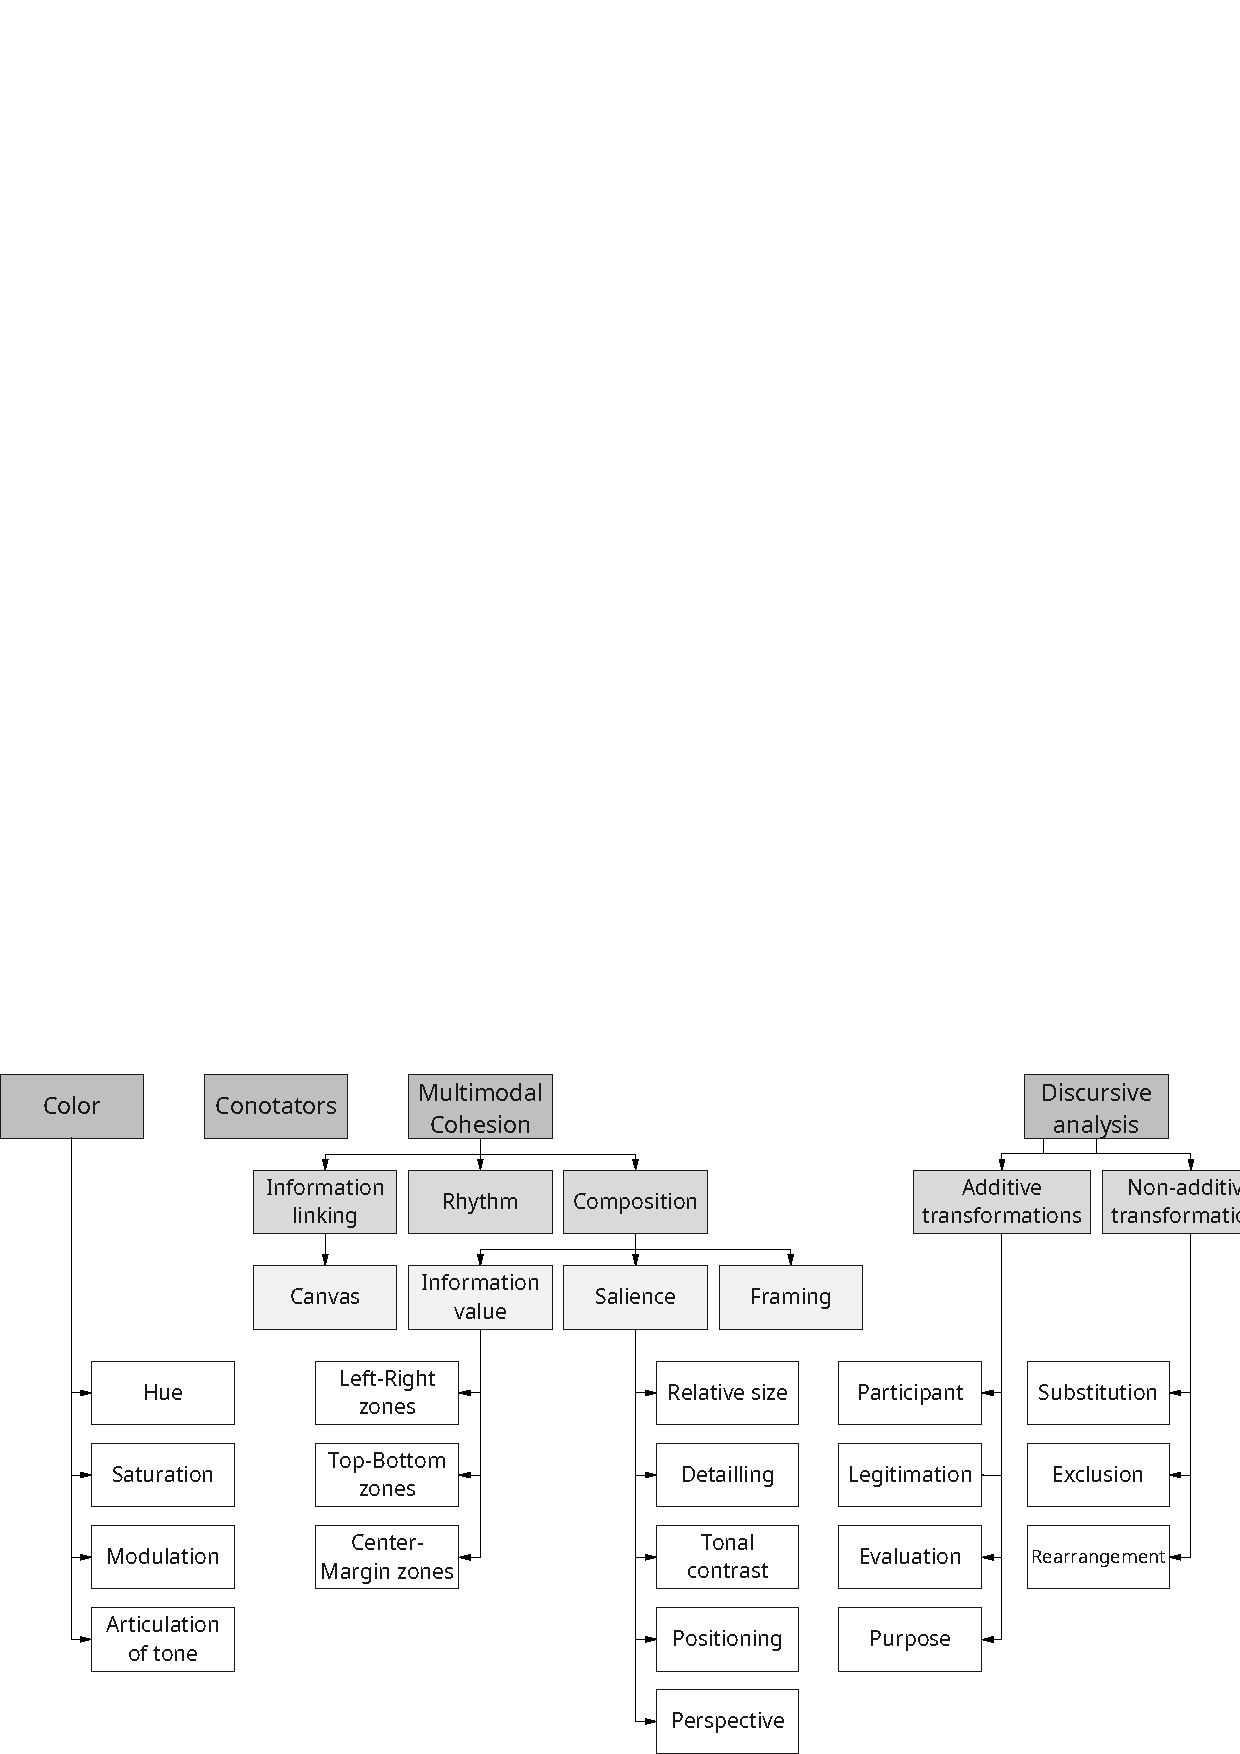
\includegraphics[width=0.75\linewidth]{fig-1.pdf}
    \caption{Percentual de estudantes que usaram IA na produção da resenha.}
    \label{fig1}
    \source{Dos autores (2025).}
\end{figure}

Esses dados expressam um valor significativo de estudantes que optaram por utilizar o ChatGPT na produção da resenha crítica neste componente em específico. Vale ressaltar que não se trata de um uso que apoia o desenvolvimento das habilidades de leitura e escrita dos estudantes, visto que as resenhas produzidas por IAG parecem ter sido geradas na íntegra, sem apresentar nenhuma marca de estilo pessoal. Porém, tão importante quanto avaliar o uso de IAG por parte dos alunos são as formas de identificação dessas práticas. Entendemos que, enquanto não houver protocolos de avaliação ou aplicações capazes de verificar o uso de linguagem generativa, é preciso refletir e elaborar essa avaliação através de esquemas experimentais, como buscamos aqui.

Tendo em vista que essa é uma prática cada vez mais comum no meio acadêmico, a preocupação dos docentes volta-se para o desenvolvimento de atividades que não possam ser realizadas pelo ChatGPT. Professores/tutores têm se dedicado a discutir e refletir sobre as práticas pedagógicas que envolvem essa temática, buscando constantemente alternativas para diversificar as tarefas e fomentar o ensino da leitura e da escrita. Contudo, as iniciativas até o momento não têm alcançado os resultados desejados, exemplos disso incluem o uso de podcasts e apresentação de tópicos em forma de vídeos, nos quais muitos alunos recorrem à IA para elaborar integralmente o roteiro, de forma que é possível apenas avaliar a sua performance diante da câmera, já que o texto é produzido por IAG. Na tentativa de avaliar, de fato, as habilidades de leitura e escrita dos estudantes, os docentes passaram a solicitar fotos de cadernos com produções textuais, mas, ainda assim, receberam trabalhos nos quais a IA gerou imagens simulando folhas de caderno e textos (outra vez, genéricos) escritos em letra cursiva.

\section{Considerações finais}\label{sec-autores}
A partir deste estudo, percebe-se que, apesar de a Inteligência Artificial ser capaz de gerar textos que, à primeira vista, parecem genuinamente humanos, ela ainda apresenta limitações que se tornam perceptíveis através de padrões lexicais e sintáticos. Isto é, ainda que a sua base de funcionamento seja composta por textos produzidos por humanos, observamos que a variabilidade das construções ainda é restrita.

Embora os resultados aqui encontrados não possam ser generalizados para todas as produções do ChatGPT – é preciso considerar que os estudantes foram convidados a resenhar textos pré-definidos, o que delimita o assunto para a IAG – acreditamos na sua relevância para a análise de textos solicitados no ambiente universitário em condições muito semelhantes às descritas neste artigo. Isso porque o chatbot opta por construções versáteis, como o uso de gerúndio e da coordenação por meio de “não apenas, mas também”, e por termos que podem ser empregados em diversos contextos por serem de significado amplo, como é o caso de “insight”. Desse modo, as categorias aqui criadas podem ser um ponto de partida para a verificação da autenticidade dos textos.

O uso indiscriminado da IA por estudantes do Ensino Superior, cria um alerta para uma possível mudança na arquitetura dos ambientes virtuais de aprendizagem e o desenvolvimento de novas práticas pedagógicas pelos docentes. Quando um aluno opta por utilizar esse recurso para produzir sua tarefa de forma integral, prejudica seu processo de aprendizagem, visto que não prioriza construir as habilidades e competências necessárias para consolidar os objetivos propostos pelo componente curricular.


\printbibliography\label{sec-bib}
% if the text is not in Portuguese, it might be necessary to use the code below instead to print the correct ABNT abbreviations [s.n.], [s.l.]
%\begin{portuguese}
%\printbibliography[title={Bibliography}]
%\end{portuguese}


%full list: conceptualization,datacuration,formalanalysis,funding,investigation,methodology,projadm,resources,software,supervision,validation,visualization,writing,review
\begin{contributors}[sec-contributors]
\authorcontribution{Róger Sullivan Faleiro}[conceptualization,datacuration,formalanalysis,methodology,supervision,visualization,writing,review]
\authorcontribution{Ana Emília Klein}[conceptualization,datacuration,formalanalysis,methodology,supervision,visualization,writing,review]
\end{contributors}


\begin{dataavailability}
\txtdataavailability{dataonly} % options: dataavailable, dataonly, databody, datanotav, nodata
\end{dataavailability}


\end{document}

